\begin{tikzpicture}[trim axis left]
\begin{axis}[
    % width of chart
    width=\textwidth,
    height=0.4\textheight,
    % no box, below chart, horizontal
    legend style={%
      draw=none,
      at={(0.5,-0.15)},
      anchor=north,
      legend columns=4,
      column sep = 1em,
      cells={align=center},
    },
    % log ticks with fixed point,
    % yticklabel={\pgfmathparse{pow(10,\tick-3)}\pgfmathprintnumber[fixed]{\pgfmathresult}}\,ms, % N ms along y-axis
    % xticklabel={\pgfmathparse{pow(5,\tick)}\pgfmathprintnumber[fixed]{\pgfmathresult}},
    xlabel near ticks,
    xlabel={Matrix size $n$ (for a Kalman filter, with $k=3n/5$)},
    ylabel near ticks,
    ylabel={Execution time of one call to Kalman filter ($\mu$s)},
    xmode = log,
    log basis x = {5},
    axis line style={opacity=0}, % hide y axis
    major tick style={draw=none}, % no ticks
    ymode=log, % log scale for y
    log basis y = {10}, % log base 10
    ymajorgrids, % rows of lines
    major grid style={gray, line width=1pt},
]

  % CBLAS
    \addplot+ [
        violet,
        mark options={fill=violet},
        error bars/.cd, y dir=both, y explicit,
    ] table [
        y error plus=ey+,
        y error minus=ey-,
    ] {
         x         y     ey+     ey-
         5        20       0      -0 
        25        70       1      -1 
       125      1118      33     -32 
       625    112024   35726  -35726 
      3125  10794507  671827 -671827 
  };

  % LT4LA
    \addplot+ [
        ForestGreen,
        mark options={fill=ForestGreen},
        error bars/.cd, y dir=both, y explicit,
    ] table [
        y error plus=ey+,
        y error minus=ey-,
    ] {
         x         y     ey+     ey-
         5        53       0       -0
        25       127      16      -11
       125      1169      20      -18
       625    105381   24608   -24608
      3125  11976659 1269467 -1269467
  };

  % Owl
    \addplot+ [
        Blue,
        mark options={fill=Blue},
        error bars/.cd, y dir=both, y explicit,
    ] table [
        y error plus=ey+,
        y error minus=ey-,
    ] {
         x         y     ey+      ey-
         5       109       1      -1
        25       157       1      -1
       125      1637      30     -23
       625    124221   38149  -38149
      3125  13326557  214388 -214388
  };

  % NumPy
    \addplot+ [
        red,
        mark options={fill=red},
        error bars/.cd, y dir=both, y explicit,
    ] table [
        y error plus=ey+,
        y error minus=ey-,
    ] {
         x         y     ey+      ey-
         5       293     17     -14
        25       355     11     -10
       125      1627     23     -20
       625    112469  11677  -11677
      3125  12702242 638344 -638344
  };

  \legend{\textsc{Cblas},\lang,\textsc{Owl},\textsc{NumPy}}

\end{axis}
\end{tikzpicture}
